% CS 5306 / INFO 5306 Project 1 report.
%
% acmart/sigconf: ships with TeX Live and Overleaf, so this compiles out of the box.
% Build: pdflatex report && bibtex report && pdflatex report && pdflatex report
%
% Every number in this file comes from out/results.json. Do not hand-edit a figure into
% the prose; if a number is wrong, the analysis is wrong.

\documentclass[sigconf,nonacm]{acmart}

\usepackage{booktabs}
\usepackage{graphicx}

% Course submission, not a real ACM paper: drop the conference furniture.
\settopmatter{printacmref=false}
\renewcommand\footnotetextcopyrightpermission[1]{}
\pagestyle{plain}

\begin{document}

\title{Feedback and Newcomer Retention in X Community Notes}
\subtitle{CS 5306 / INFO 5306, Project 1}

\author{Kevin Lei}
\affiliation{\institution{Cornell University}\country{}}
\email{kl2344@cornell.edu}

\author{Kyungmin Nam}
\affiliation{\institution{Cornell University}\country{}}
\email{kn467@cornell.edu}

\author{Brittany Sun}
\affiliation{\institution{Cornell University}\country{}}
\email{bs835@cornell.edu}

\begin{abstract}
In X's Community Notes, a contributor's first note can be rated Helpful, rated Not
Helpful, or sit unresolved in ``Needs More Ratings'' indefinitely. We ask whether an
explicit rejection predicts departure differently from never receiving a verdict at all,
a comparison the Wikipedia newcomer literature cannot make. Using a full public snapshot
of 3.1 million notes and classifying each first note by the status it held seven days
after it was written, we find that contributors rejected within seven days were
$15.0$ percentage points less likely to write again within thirty days than contributors
whose note was still unresolved ($95\%$ CI $-15.5$ to $-14.5$). That figure is mostly not
discouragement. In April 2024 X began revoking writing ability after a single Not Helpful
note, and the gap triples across that date, from $6.1$ to $17.1$ points; $89.4\%$ of
rejected first-time authors have since lost writing ability, typically the same day the
verdict arrived. Cohorts predating the rule, who could not be locked out, still show a
gap of about five points. We report that residual as the defensible estimate, and the
pooled figure as an artifact of a design decision the platform made.
\end{abstract}

\maketitle

\section{Introduction}

Crowdsourced moderation systems depend on newcomers who stay. Community Notes asks
volunteers to write short corrections on posts, then has other volunteers rate them. A
matrix-factorization scorer publishes a note only when contributors who usually disagree
agree it is helpful~\cite{wojcik2022birdwatch}. The system is deliberately hard to satisfy,
and most notes never satisfy it.

That produces an outcome structure with no clean analogue elsewhere. A first note can be
rated Helpful, rated Not Helpful, or receive no verdict at all, remaining in ``Needs More
Ratings'' (NMR) for as long as it exists. Wikipedia's newcomer literature has established
that early negative feedback predicts departure: reverting a newcomer's first edit
measurably reduces the chance they edit again~\cite{halfaker2011newbies,halfaker2013rise}.
But on Wikipedia an edit that is not reverted stands. There is no large population of
contributors whose first contribution was met with silence in the way that most Community
Notes contributions are.

\textbf{Our question is whether explicit rejection predicts different retention than
getting no verdict at all.} Not Helpful versus NMR is the comparison; Helpful is a
reference point. This matters for design, because a system whose modal outcome is ``no
decision yet'' is making an implicit choice about how to treat newcomers, and it is not
obvious whether silence is gentler than rejection or worse.

The answer turned out to depend on something we did not anticipate. Rejected contributors
are far less likely to return --- but for most of the period we study, rejection does not
merely discourage a contributor, it mechanically strips their ability to write. Separating
the two is the substance of this paper, and Section~\ref{sec:lockout} is where we do it.
The short version: an explicit Not Helpful verdict predicts sharply lower continued
contribution than no verdict, most of that gap is the platform's writing lockout rather
than discouragement, and a smaller association of roughly five points survives in cohorts
that predate the lockout rule.

\section{The System}
\label{sec:system}

Two mechanics shape everything that follows.

\textbf{Contributors earn the ability to write by rating first.} New contributors may only
rate. They unlock writing by reaching a Rating Impact of $5$, earned by rating notes before
they reach a status and matching the status they go on to reach~\cite{communitynoteswriting}.
This requirement was introduced in September 2022 and applies to every cohort we analyse.
\emph{Our ``newcomers'' are therefore newcomers to writing only.} Each had already rated
enough notes, accurately and early enough, to clear a quality bar. This weakens the analogy
to Wikipedia newcomers, where no comparable filter exists, and it means our population is
more committed than a typical first-time participant.

\textbf{Not Helpful ratings can cost a contributor the ability to write.} A contributor's
writing ability is locked when three of their last five resolved notes are Not Helpful ---
or, since 2 April 2024, when \emph{any} note reaches Not Helpful while their Writing Impact
is zero or negative~\cite{communitynoteswriting}. Writing Impact starts at zero and only
moves when a note resolves. A first-time author therefore has a Writing Impact of exactly
zero, so from April 2024 onward a single Not Helpful first note locks writing on its own,
while a first note sitting in NMR does nothing. The contrast this paper measures is a
contrast the platform itself acts on. We return to this in Section~\ref{sec:lockout}.

A note's status is not permanent, and statuses are recomputed periodically, but the public
data records when each note first left NMR and what it became~\cite{communitynotesranking}.
That first transition is what we use.

\section{Related Work}

The closest body of work is on Wikipedia newcomer retention. Halfaker et
al.~\cite{halfaker2011newbies} show across 400,000 revisions that having an early edit
reverted is powerfully demotivating, reducing the volume of subsequent work, while still
improving aggregate quality --- the system gains more from rejecting bad work than it loses
by driving away the people who did it. The later account of Wikipedia's
decline~\cite{halfaker2013rise} attributes much of it to increasingly automated and
impersonal rejection of newcomers.

Community Notes differs in two ways that make it a useful contrast. Rejection is the output
of a scoring rule rather than a person's judgment, so a rejected contributor has no editor
to argue with and no revert summary to read. And the modal outcome is neither acceptance
nor rejection but silence, which Wikipedia does not produce at comparable scale. Recent
descriptive work covers the program's first four years, including contributor activity and
rating behaviour~\cite{mohammadi2025birdwatch}, but not, to our knowledge, the retention
consequences of the no-verdict condition.

\section{Data}
\label{sec:data}

We use the public Community Notes bulk downloads~\cite{communitynotesdata}, snapshot dated
\textbf{18 September 2026}. Each snapshot is cumulative back to 2021, so one is enough.
Upstream keeps roughly a week of snapshots and older dates return 404, so the archive we
took locally is the only copy; nothing in our pipeline writes to it.

\begin{sloppypar}
Three tables: \texttt{notes} ($3{,}086{,}867$ rows), \texttt{noteStatusHistory}
($3{,}290{,}294$ rows), and \texttt{userEnrollment} ($1{,}490{,}672$ rows). The project
rests on two fields in the second: \texttt{firstNonNMRStatus}, the first real verdict a
note received, and \texttt{timestampMillisOf\-FirstNonNMRStatus}, when it arrived. Both
are
empty when a note never left NMR, which is true of $82.7\%$ of notes.
\end{sloppypar}

Snapshots contain only notes created up to 48 hours before release, so the effective data
cutoff is \textbf{16 September 2026}, two days before the snapshot date. All censoring uses
the cutoff, not the snapshot date.

We did not use the \texttt{ratings} table, which runs to tens of gigabytes and answers a
different question --- we need note outcomes, not individual ratings --- or the text of the
annotated posts, which is not public.

\textbf{Author identifier stability.} Our analysis assumes a participant identifier means
the same person across releases. Because snapshots expire, this can only be checked while a
second one is still downloadable, so we did it: comparing \texttt{noteStatusHistory} across
the 18 and 16 September releases gives $3{,}282{,}773$ notes present in both and
\textbf{zero} author-identifier mismatches.

\textbf{Two data problems we found rather than assumed.} First,
\texttt{firstNonNMRStatus} is not merely sparse before May 2022, it is \emph{empty}: not one
of the $28{,}988$ notes created before then has a recorded verdict. Those cohorts are
$100\%$ NMR by construction, not by outcome. Second, $233{,}514$ notes ($7.6\%$) have no
\texttt{noteStatusHistory} row at all, spread across 28 months from March 2024 onward at a
rate rising from $6.7\%$ to $14.1\%$. Those notes have \emph{no recorded outcome}, which is
not the same as never leaving NMR; treating them as NMR would inflate the comparison group
by a growing amount and manufacture a cohort trend. Both drive exclusions in
Section~\ref{sec:exclusions}.

\section{Method}
\label{sec:method}

\subsection{Contributor-level dataset}

We join \texttt{notes} to \texttt{noteStatusHistory} on note identifier and emit one row per
author: their first note, its outcome and timing, their next note, their cohort month, and
first-note features (classification, whether it cites a URL, length, reason tags). A first
note is the author's earliest note in the snapshot, ties broken by note identifier so the
ordering is total and the build deterministic. Since snapshots are cumulative back to 2021,
that is genuinely their first note. The table has $343{,}176$ rows, one per distinct author
in \texttt{notes}.

Before using it we validated it against the raw files: twelve structural checks, plus twenty
randomly sampled authors rebuilt field by field from the raw TSVs by a separate Python
parser that does not go through our query engine. All twelve checks and all twenty authors
matched.

\subsection{Landmark classification}
\label{sec:landmark}

This is the central methodological choice. \textbf{We classify each first note by the status
it held seven days after it was written}, not by the status it eventually reached.

Classifying by eventual status uses information that did not exist when the contributor
decided whether to come back. A note that sat in NMR for three months and then turned Not
Helpful was, for the entire period in which the contributor was deciding, a note with no
verdict. Worse, the eventual-status NMR group is partly a function of when the snapshot was
taken rather than of anything the contributor experienced.

Seven days is generous. From 2023 onward, the median first note reaches a verdict in under a
third of a day and the ninetieth percentile inside two days, so a seven-day landmark
captures nearly every verdict that will ever arrive. We also drop authors who wrote again
\emph{before} day seven: no feedback could have reached them, so their return says nothing
about how they reacted to one. A verdict landing after day seven counts as NMR here, by
design.

\subsection{Retention and censoring}

Retention is whether the author wrote another note between the landmark and the end of a
30-, 60-, or 90-day window. An author enters a window only if the entire window closes
before the data cutoff, so each window has its own sample size. Proportions carry Wilson
$95\%$ intervals and differences carry Newcombe hybrid-score intervals.

Section~\ref{sec:survival} reports Kaplan-Meier curves instead, which censor rather than
discard, as a check that the windowing is not doing the work.

\subsection{Exclusions}
\label{sec:exclusions}

Exclusions are boolean columns applied in one place, never deleted rows. Of $343{,}176$
authors we keep $322{,}094$:

\begin{itemize}
  \item $5{,}052$ authors in cohorts before January 2023, where verdicts are absent or were
        rewritten by a January 2023 rescoring of all historical notes.
  \item $15{,}997$ authors whose first note has no status-history row, whose outcome is
        unknown rather than absent.
  \item $35$ AI note-writer accounts, identified by an enrollment state prefixed
        \texttt{api}. They are negligible as authors but wrote $8.6\%$ of all notes, and an
        AI that stops writing has not given up.
\end{itemize}

Applying the landmark leaves $230{,}588$ authors observable at day seven, of whom
$227{,}324$ have a fully observed 30-day window.

\section{Results}
\label{sec:results}

\textbf{Contributors whose first note was rated Not Helpful within seven days were $15.0$
percentage points less likely to write another note in the following thirty days than
contributors whose first note was still unresolved} ($95\%$ CI $-15.5$ to $-14.5$;
$n=19{,}153$ Not Helpful and $183{,}373$ NMR). Section~\ref{sec:lockout} explains why that
number is mostly not what it appears to be.

\begin{table}[t]
  \caption{Retention by first-note outcome at day 7. Wilson 95\% intervals.}
  \label{tab:primary}
  \begin{tabular}{lrrr}
    \toprule
    First-note outcome & $n$ & 30-day & 90-day \\
    \midrule
    Helpful          & 24,798  & 27.6\% & 43.7\% \\
    Not Helpful      & 19,153  & 10.6\% & 19.3\% \\
    No verdict (NMR) & 183,373 & 25.6\% & 41.4\% \\
    \bottomrule
  \end{tabular}
\end{table}

\begin{figure}[t]
  \centering
  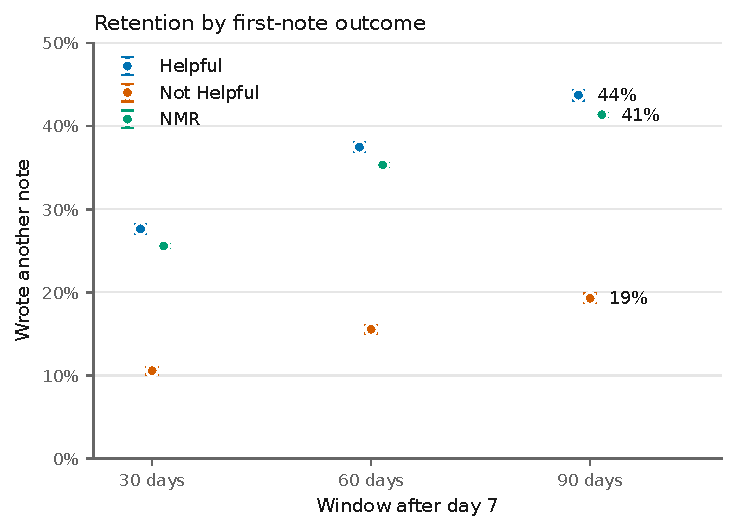
\includegraphics[width=\columnwidth]{../out/figures/fig2_retention.pdf}
  \caption{Retention by first-note outcome at 30, 60, and 90 days, with 95\% intervals.}
  \label{fig:retention}
\end{figure}

\subsection{The Not Helpful versus no-verdict comparison}

Table~\ref{tab:primary} and Figure~\ref{fig:retention} show the answer to the paper's
question, and the shape is asymmetric. Rejection is associated with a large deficit:
$-15.0$ points at thirty days, widening to $-22.1$ at ninety. Approval is associated with
almost nothing: $+2.1$ points at thirty days and $+2.4$ at ninety. Getting no verdict at all
is, on these numbers, nearly as good as being told your note was helpful.

\textbf{The specification matters more than we expected.} Computed the obvious way ---
labelling each note with whatever verdict it eventually received and measuring retention from
the note itself --- the same data gives $-21.1$ points, overstating the difference by $6.1$
points. Most of that comes from keeping the authors who wrote again within the week, the most
engaged people in the sample, without asking whether any feedback had reached them. We hold
censoring identical between the two so the comparison isolates the landmark. That the easy
specification is wrong by forty percent is itself worth reporting.

\subsection{Cohorts, and a structural break}
\label{sec:lockout}

Splitting by cohort month changes the finding. Figure~\ref{fig:cohort} shows the gap is small
and often indistinguishable from zero through 2023 and early 2024, then collapses. Not Helpful
retention falls from around $28\%$ in February 2024 to $9.6\%$ in April 2024 and stays in a
$3$--$8\%$ band thereafter, while the other two groups drift down together and far more
gently. Pooled either side of that date, the Not Helpful minus NMR gap is $-6.1$ points before
April 2024 ($95\%$ CI $-7.4$ to $-4.7$) and $-17.1$ points after ($-17.6$ to $-16.7$).

April 2024 is when X began locking writing ability on a single Not Helpful note
(Section~\ref{sec:system}). The enrollment data confirms the mechanism directly:
\textbf{$89.4\%$ of rejected first-time authors have lost writing ability at least once},
against $16.8\%$ of the no-verdict group, and $48.7\%$ are still locked out. Among rejected
authors who wrote exactly one note and have been locked out, the median gap between the
verdict arriving and the lockout is $0.03$ days and $84.0\%$ were locked within a week. The
verdict and the lockout are effectively the same event.

\begin{figure*}[t]
  \centering
  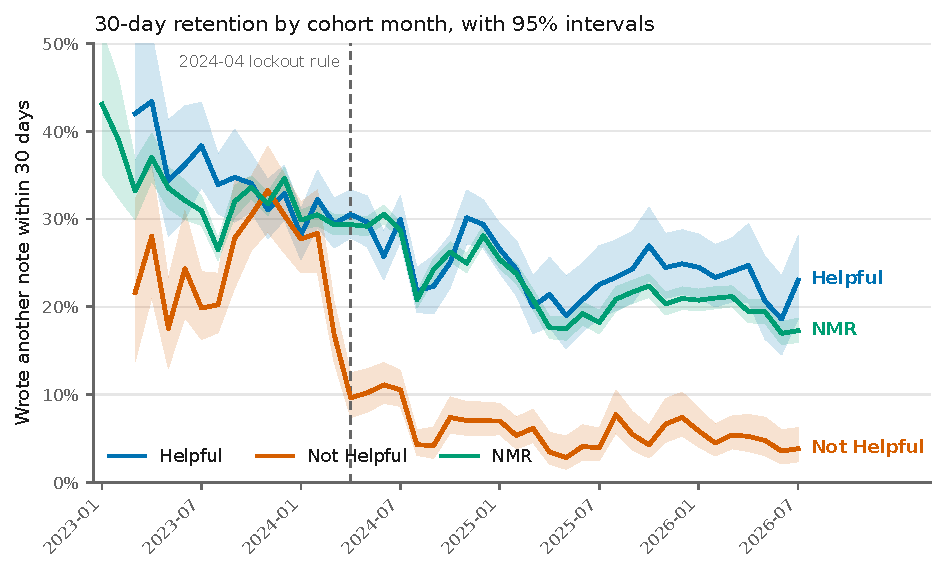
\includegraphics[width=0.82\textwidth]{../out/figures/fig3_cohorts.pdf}
  \caption{30-day retention by cohort month and first-note outcome, with 95\% intervals. The
  dashed line marks April 2024, when a single Not Helpful note began locking writing ability.
  Cohort months too recent for a 30-day window to close before the data cutoff are omitted.}
  \label{fig:cohort}
\end{figure*}

\textbf{This does not reduce the finding to zero.} The enrollment field records only a
contributor's most recent lockout, so a 2023 author's could have occurred years later under
the new rule. Counting only lockouts stamped before the rule date, just $1.2\%$ of pre-rule
rejected authors had lost writing ability when it mattered, against $0.3\%$ of the no-verdict
group. Those cohorts really were free to keep writing, and they still show a $6.1$-point gap.
Even if every locked contributor would otherwise have returned, at most $1.2$ points of that
is mechanical, leaving \textbf{roughly five points that is not}.

We therefore report two numbers with different jobs. The pooled $-15.0$ points describes what
happens to rejected newcomers in Community Notes today, and is mostly the platform's lockout
doing what it was designed to do. The $-4.9$ points from pre-rule cohorts is our estimate of
the association between rejection and departure absent that mechanism.

\subsection{Time to return}
\label{sec:survival}

Kaplan-Meier estimates agree with the windowed proportions and rule out the windowing as an
artifact. Follow-up starts at the day-7 landmark, the event is the author's next note, and
authors who never return are censored at the data cutoff rather than dropped. By day ninety
$43.7\%$ of Helpful authors, $41.2\%$ of NMR authors and $19.0\%$ of Not Helpful authors have
returned, within half a point of the windowed figures in Table~\ref{tab:primary}. No group
reaches a median time to return within ninety days --- most contributors never write a second
note at all.

\subsection{Adjusted estimates}

A logistic regression of 30-day retention on day-7 status, with cohort-month fixed effects and
first-note controls (classification, URL presence, length, and reason tags), gives an odds
ratio of $0.36$ for Not Helpful ($95\%$ CI $0.34$--$0.38$), an average marginal effect of
$-18.5$ points. That is $3.5$ points larger than the raw difference, not smaller. The reason is
Section~\ref{sec:lockout}: cohort fixed effects make the comparison within cohort, which
removes the early cohorts' smaller gaps from the average. We report both rather than the more
convenient one. One control is worth noting: a first note asserting a post is \emph{not}
misleading is associated with $+2.5$ points of retention once status is held constant, despite
such notes being structurally ineligible for Helpful status and reaching Not Helpful far more
often.

\section{Robustness}

Table~\ref{tab:robust} reruns the primary comparison under each variation. The difference is
negative in all six, ranging from $-5.7$ to $-18.2$ points against a baseline of $-15.0$, with
no sign flips. Moving the landmark trades sample composition against classification accuracy in
the expected direction. The stricter retention definition compresses the difference because base
rates fall for every group. Nothing here is close to the sensitivity that matters, which is the
cohort split.

\begin{table}[t]
  \caption{Not Helpful minus NMR difference at 30 days under each variation.}
  \label{tab:robust}
  \begin{tabular}{lr}
    \toprule
    Variation & Difference \\
    \midrule
    Baseline (day-7 landmark)             & $-15.0$ pp \\
    Landmark at 3 days                    & $-18.2$ pp \\
    Landmark at 14 days                   & $-11.7$ pp \\
    Excluding not-misleading first notes  & $-14.0$ pp \\
    Retention = two or more later notes   & $-5.7$ pp \\
    Cohorts with 90+ days after the window& $-15.0$ pp \\
    \midrule
    Naive eventual-status specification   & $-21.1$ pp \\
    \bottomrule
  \end{tabular}
\end{table}

\section{Threats to Validity}
\label{sec:threats}

\textbf{Writing lockouts.} The largest threat, and the one that reshaped the paper. We have
bounded it in Section~\ref{sec:lockout} rather than dismissed it, but the bound is one-sided.
\texttt{userEnrollment} carries one current state per contributor with no history, so after
April 2024 we cannot separate a contributor who was locked at the moment they would have written
from one who had already lost interest. An author who was locked, earned back in, and left anyway
is indistinguishable from one never locked. Our pre-rule estimate sidesteps this by using a period
when the mechanism did not exist, at the cost of a smaller and older sample.

\textbf{Selection.} We did not assign anyone to Not Helpful or NMR. A weak first note plausibly
produces both a bad verdict and a contributor who was leaving regardless. Controlling for
observable note features is not the same as solving this, and we claim association throughout.

\textbf{Notification.} We do not observe whether a contributor ever saw their note's status. The
landmark assumes seven days is enough for feedback to arrive, which is a claim about the system's
notifications that we cannot verify from public data.

\textbf{Survivorship.} Deleted notes disappear from \texttt{notes} while remaining in
\texttt{noteStatusHistory}, so our author population is drawn from surviving notes only.

\textbf{Automated authors.} AI note writers entered the system in 2025 and are excluded, but
only via current enrollment state; an account since moved to another state would be invisible.

\section{What We Did}
\label{sec:work}

Four weeks, three people, and the work was mostly not the statistics.

The first week went on establishing what the system actually does, which turned out to be the
highest-value thing we did. Reading the scoring source alongside the published guide is what
surfaced the April 2024 lockout rule and, critically, its \emph{date} --- which is what later let
us separate the mechanism from the behaviour instead of writing a paragraph apologising for the
confound. The guide's rendered pages are client-side rendered and return nothing to a plain
fetch, so we worked from the markdown sources the site is built from.

The second week went on the data, and produced two stops. We found that first-verdict fields are
entirely empty before May 2022, which killed the 2021--2022 cohorts outright, and that $7.6\%$ of
notes have no status-history row at all, which is undocumented and would have silently inflated
our comparison group at a rate that grows over time. Both were flagged and escalated rather than
patched around, which cost a day each and was worth it. We also verified author-identifier
stability across two releases inside the one-week window during which that check is possible at
all.

Infrastructure bit in small ways worth recording. The Python environment is a pinned Nix flake;
an initial attempt with \texttt{uv} failed because its downloaded interpreter is dynamically
linked against a loader that does not exist on NixOS. The survival library we planned to use does
not build against the pinned package set, so Kaplan-Meier and the log-rank test are computed with
\texttt{statsmodels} instead. Loading the tables with default CSV quoting silently corrupts rows,
because note text contains bare double quotes.

Two mistakes we caught ourselves. Drawing the cohort figure revealed that the most recent month
spikes in every series, because only authors who joined in the first days of that month can have a
30-day window close before the cutoff --- a biased slice, not a cohort. We fixed it in the analysis
with an explicit completeness flag rather than trimming the chart. And our first pass at the
regression writeup claimed the adjusted and raw estimates agreed, when they differ by $3.5$ points;
the honest explanation of \emph{why} they differ turned out to be more informative than the
agreement would have been.

Reproducibility was a constraint throughout rather than an afterthought. The contributor table was
frozen after validation and never rebuilt. Exclusions live in one function. Every number in this
paper is generated into a single JSON file that the paper quotes, so no figure here was typed by
hand.

\section{Conclusion}

An explicit Not Helpful verdict on a first note predicts substantially lower continued
contribution than no verdict at all --- $15.0$ points at thirty days --- but most of that is X's
writing lockout rather than contributors choosing to leave. In cohorts predating the lockout rule,
where rejection carried no mechanical penalty, the association is about five points. Rejection
discourages, modestly; the platform then removes the option entirely, which is what the pooled
number mostly measures.

The result we did not expect is the asymmetry. Approval buys almost nothing: contributors told
their note was Helpful returned only about two points more often than contributors told nothing at
all. For a system whose modal outcome is silence, that is reassuring in one way and troubling in
another. Silence is not experienced as rejection, so the $82.7\%$ of notes that never resolve are
not quietly driving people away. But the system also gets very little retention benefit from
telling someone they did well. If Community Notes wants newcomers to stay, the lever is not
faster verdicts --- it is reconsidering whether a first rejection should cost someone the ability
to try again, given that $89.4\%$ of rejected first-time authors lose it, usually the same day.

\bibliographystyle{ACM-Reference-Format}
\bibliography{refs}

\end{document}
